% Compile with: pdflatex lectures_34_35.tex
% Requires: amsmath, amssymb, amsthm, mathtools, xcolor, mdframed,
%           enumitem, hyperref, pagecolor, microtype, tikz

\documentclass[11pt]{article}
\usepackage[margin=1in]{geometry}
\usepackage{amsmath, amssymb, amsthm}
\usepackage{mathtools}
\usepackage{xcolor}
\usepackage{mdframed}
\usepackage{enumitem}
\usepackage{hyperref}
\usepackage{pagecolor}
\usepackage{microtype}
\usepackage{tikz}
\usetikzlibrary{arrows.meta, positioning, shapes.geometric}

% ----- Colour palette -----
\definecolor{cream}{HTML}{FFFDF5}
\definecolor{defblue}{HTML}{1A4A7A}
\definecolor{thmgreen}{HTML}{1A5C3A}
\definecolor{warnAmber}{HTML}{7A4A00}
\definecolor{dangerRed}{HTML}{7A1A1A}
\definecolor{boxbluebg}{HTML}{EBF3FB}
\definecolor{boxgreenbg}{HTML}{EBF7EF}
\definecolor{boxamberbg}{HTML}{FDF5E6}
\definecolor{boxredbg}{HTML}{FBEBEB}
\pagecolor{cream}

% ----- Theorem styles -----
\newtheoremstyle{defstyle}    {8pt}{8pt}{\normalfont}{0pt}{\bfseries\color{defblue}} {.}{0.5em}{}
\newtheoremstyle{thmstyle}    {8pt}{8pt}{\normalfont}{0pt}{\bfseries\color{thmgreen}}{.}{0.5em}{}
\newtheoremstyle{notstyle}    {8pt}{8pt}{\normalfont}{0pt}{\bfseries\color{warnAmber}}{.}{0.5em}{}
\newtheoremstyle{cautionstyle}{8pt}{8pt}{\normalfont}{0pt}{\bfseries\color{dangerRed}}{.}{0.5em}{}

\theoremstyle{defstyle}
\newtheorem{definition}{Definition}[section]

\theoremstyle{thmstyle}
\newtheorem{theorem}{Theorem}[section]
\newtheorem{corollary}[theorem]{Corollary}

\theoremstyle{notstyle}
\newtheorem*{remark}{Remark}
\newtheorem*{example}{Example}

\theoremstyle{cautionstyle}
\newtheorem*{caution}{Caution}

% ----- Boxes -----
\newmdenv[
  backgroundcolor=boxbluebg, linecolor=defblue, linewidth=2pt,
  topline=false, rightline=false, bottomline=false,
  innerleftmargin=10pt, innerrightmargin=10pt,
  innertopmargin=6pt, innerbottommargin=6pt,
  skipabove=8pt, skipbelow=8pt
]{defbox}

\newmdenv[
  backgroundcolor=boxgreenbg, linecolor=thmgreen, linewidth=2pt,
  topline=false, rightline=false, bottomline=false,
  innerleftmargin=10pt, innerrightmargin=10pt,
  innertopmargin=6pt, innerbottommargin=6pt,
  skipabove=8pt, skipbelow=8pt
]{thmbox}

\newmdenv[
  backgroundcolor=boxamberbg, linecolor=warnAmber, linewidth=2pt,
  topline=false, rightline=false, bottomline=false,
  innerleftmargin=10pt, innerrightmargin=10pt,
  innertopmargin=6pt, innerbottommargin=6pt,
  skipabove=8pt, skipbelow=8pt
]{notebox}

\newmdenv[
  backgroundcolor=boxredbg, linecolor=dangerRed, linewidth=2pt,
  topline=false, rightline=false, bottomline=false,
  innerleftmargin=10pt, innerrightmargin=10pt,
  innertopmargin=6pt, innerbottommargin=6pt,
  skipabove=8pt, skipbelow=8pt
]{cautionbox}

% ----- Macros -----
\newcommand{\Z}{\mathbb{Z}}
\newcommand{\N}{\mathbb{N}}
\newcommand{\R}{\mathbb{R}}

\begin{document}

\begin{center}
  {\Large\bfseries Lectures 34 \& 35 --- Graphs, Degree, and the Handshaking Lemma}\\[4pt]
  {\normalsize CS 173: Discrete Structures \quad$\cdot$\quad Graph Theory}\\[2pt]
  {\small\color{gray} University of Illinois at Urbana-Champaign}
\end{center}
\vspace{1em}\hrule\vspace{1.5em}

\section{Defining a graph}

A graph is a combinatorial object built from two ingredients: a collection
of \emph{points} (called vertices or nodes) and a collection of
\emph{connections} between pairs of those points (called edges). Both
ingredients are sets, the vertex set is required to be finite, and the only
structural constraint is that every edge is a $2$-element subset of the
vertex set.

\begin{defbox}
\begin{definition}[Graph]
A \textbf{graph} $G$ is determined by
\begin{itemize}[leftmargin=2em, itemsep=2pt]
  \item a \emph{finite} set of \emph{nodes} (or \emph{vertices}) $V(G)$, and
  \item a set of \emph{edges} $E(G)$,
\end{itemize}
such that
\[
  E(G) \;\subseteq\; \bigl\{\, W \;\bigm|\; W \subseteq V(G) \,\wedge\, |W| = 2 \,\bigr\}.
\]
\end{definition}
\end{defbox}

The symbol $G$ in $V(G)$ and $E(G)$ is the \emph{name of the graph}; the
functions $V(\cdot)$ and $E(\cdot)$ extract the vertex set and edge set of
whichever graph you name. Read $V(G)$ as ``the vertex set of $G$'' and
$E(G)$ as ``the edge set of $G$.''

\begin{notebox}
\begin{remark}
The condition $E(G) \subseteq \{ W \mid W \subseteq V(G) \wedge |W| = 2 \}$
is doing a lot of work. Unpacking it:
\begin{itemize}[leftmargin=2em, itemsep=2pt]
  \item Each edge is a \emph{set} $W$, not an ordered pair, so
        $\{0, 1\} = \{1, 0\}$ denotes a single edge. This is the formal
        reason these graphs are \textbf{undirected}.
  \item $W \subseteq V(G)$ forces both endpoints to be vertices of $G$.
  \item $|W| = 2$ forces the two endpoints to be \emph{distinct}, ruling
        out loops $\{v, v\} = \{v\}$ (which has cardinality $1$, not $2$).
  \item $E(G)$ is itself a set, so no edge is repeated --- this rules out
        parallel edges (multigraphs).
\end{itemize}
Finiteness of $V(G)$ then forces $E(G)$ to be finite as well, since
$E(G) \subseteq \mathcal{P}(V(G))$ and the power set of a finite set is
finite.
\end{remark}
\end{notebox}

\begin{cautionbox}
\begin{caution}
A graph is determined by the \emph{pair} $(V(G), E(G))$, not by $E(G)$
alone. Two graphs can have the same edge set but different vertex sets if
one of them has \emph{isolated} vertices --- vertices in $V(G)$ that appear
in no edge.
\end{caution}
\end{cautionbox}

\section{First example}

\begin{notebox}
\begin{example}
Let $G$ be the graph with
\[
  V(G) = \{0, 1, 2\}, \qquad
  E(G) = \bigl\{ \{0, 1\},\ \{1, 2\} \bigr\}.
\]
Each element of $E(G)$ is a $2$-element subset of $V(G)$, so the definition
is satisfied.
\end{example}
\end{notebox}

\begin{center}
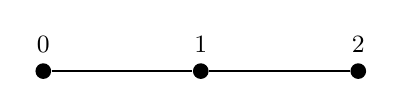
\begin{tikzpicture}[every node/.style={font=\small}]
  \tikzset{dot/.style={circle, fill, inner sep=2pt}}
  \node[dot, label=above:{$0$}] (a) at (0, 0) {};
  \node[dot, label=above:{$1$}] (b) at (2, 0) {};
  \node[dot, label=above:{$2$}] (c) at (4, 0) {};
  \draw[thick] (a) -- (b);
  \draw[thick] (b) -- (c);
\end{tikzpicture}
\end{center}

\noindent
The vertex $1$ is shared by both edges; vertices $0$ and $2$ each belong to
exactly one edge, and there is no edge directly between $0$ and $2$.

\section{Neighbourhood and incident edges}

Once a graph $G$ and a vertex $v \in V(G)$ are fixed, two natural ``local''
sets describe how $v$ sits inside $G$: the other vertices it is joined to,
and the edges that touch it. The first lives in $V(G)$, the second in
$E(G)$.

\begin{defbox}
\begin{definition}[Neighbourhood]
Given a graph $G$ and a node $v \in V(G)$, the \textbf{neighbourhood} of
$v$ in $G$ is
\[
  N_G(v) \;:=\; \bigl\{\, w \in V(G) \;\bigm|\; \{v, w\} \in E(G) \,\bigr\}.
\]
That is, $N_G(v)$ is the set of vertices joined to $v$ by an edge.
\end{definition}
\end{defbox}

\begin{defbox}
\begin{definition}[Incident edges]
Given a graph $G$ and a node $v \in V(G)$, the set of \textbf{edges
incident to} $v$ is
\[
  I_G(v) \;:=\; \bigl\{\, e \in E(G) \;\bigm|\; v \in e \,\bigr\}.
\]
That is, $I_G(v)$ is the set of edges that have $v$ as one of their two
endpoints.
\end{definition}
\end{defbox}

The two sets answer different questions, and the type-checking matters:

\begin{center}
\renewcommand{\arraystretch}{1.5}
\begin{tabular}{|l|l|l|}
\hline
\textbf{Set} & \textbf{Element type} & \textbf{Lives in} \\
\hline
$N_G(v)$ & a \emph{vertex} $w$ adjacent to $v$ & $\mathcal{P}(V(G))$ \\
$I_G(v)$ & an \emph{edge} $e$ containing $v$    & $\mathcal{P}(E(G))$ \\
\hline
\end{tabular}
\end{center}

\noindent
The two are tightly linked: each $e \in I_G(v)$ has the form $e = \{v, w\}$
for exactly one $w \in N_G(v)$, and conversely each $w \in N_G(v)$
corresponds to a unique edge $\{v, w\} \in I_G(v)$. So
$|N_G(v)| = |I_G(v)|$ for every vertex.

\begin{cautionbox}
\begin{caution}
$v \notin N_G(v)$. The neighbourhood of $v$ never contains $v$ itself,
because $\{v, v\} = \{v\}$ has cardinality $1$, so it is not a valid edge.
Some texts use $N_G[v] = N_G(v) \cup \{v\}$ for the \emph{closed}
neighbourhood; the version on the board is the \emph{open} neighbourhood
and excludes $v$.
\end{caution}
\end{cautionbox}

\section{Worked example}

The board showed a five-vertex graph $G$ to compute $N_G$ and $I_G$ on a
less trivial picture. Let
\[
  V(G) = \{a, b, c, d, e\}, \qquad
  E(G) = \bigl\{ \{a,b\},\ \{a,c\},\ \{a,e\},\ \{b,c\} \bigr\}.
\]
The vertex $d$ is in $V(G)$ but is not an endpoint of any edge --- it is an
\emph{isolated} vertex, the canonical illustration of why $V(G)$ cannot be
recovered from $E(G)$.

\begin{center}
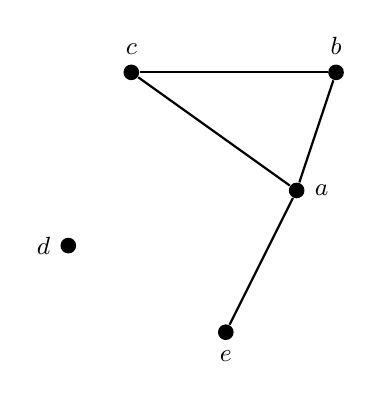
\begin{tikzpicture}[every node/.style={font=\small}]
  \tikzset{dot/.style={circle, fill, inner sep=2pt}}
  \node[dot, label=above:{$c$}] (c) at (-1.6, 1.8) {};
  \node[dot, label=above:{$b$}] (b) at ( 1.0, 1.8) {};
  \node[dot, label=right:{$a$}] (a) at ( 0.5, 0.3) {};
  \node[dot, label=left:{$d$}]  (d) at (-2.4,-0.4) {};
  \node[dot, label=below:{$e$}] (e) at (-0.4,-1.5) {};
  \draw[thick] (c) -- (b);
  \draw[thick] (a) -- (b);
  \draw[thick] (a) -- (c);
  \draw[thick] (a) -- (e);
\end{tikzpicture}
\end{center}

\noindent
Reading off the neighbourhood and incident-edge sets at $a$:
\[
  N_G(a) = \{b,\, c,\, e\},
  \qquad
  I_G(a) = \bigl\{\, \{a,b\},\ \{a,c\},\ \{a,e\} \,\bigr\}.
\]
Both have size $3$, consistent with $|N_G(v)| = |I_G(v)|$. The remaining
vertices:
\begin{align*}
  N_G(b) &= \{a, c\},      & I_G(b) &= \bigl\{\{a,b\},\{b,c\}\bigr\}, \\
  N_G(c) &= \{a, b\},      & I_G(c) &= \bigl\{\{a,c\},\{b,c\}\bigr\}, \\
  N_G(d) &= \varnothing,   & I_G(d) &= \varnothing, \\
  N_G(e) &= \{a\},         & I_G(e) &= \bigl\{\{a,e\}\bigr\}.
\end{align*}

\section{Degree of a vertex}

The number of edges touching a vertex is so fundamental that it gets its
own name. Because every graph $G$ assigns a single non-negative integer
to each vertex, degree is presented as a \emph{function} from $V(G)$ into
$\N$ --- well-defined because $V(G)$ is finite, hence so is each
$I_G(v)$.

\begin{defbox}
\begin{definition}[Degree]
Given a graph $G$, the \textbf{degree} function
\[
  \deg_G \colon V(G) \to \N
\]
is defined, for any $v \in V(G)$, by
\[
  \deg_G(v) \;:=\; \bigl|\, I_G(v) \,\bigr| \;=\; \bigl|\, N_G(v) \,\bigr|.
\]
That is, $\deg_G(v)$ is the number of edges incident to $v$, equivalently
the number of neighbours of $v$. The two counts agree because the
correspondence $w \mapsto \{v, w\}$ is a bijection between $N_G(v)$ and
$I_G(v)$.
\end{definition}
\end{defbox}

\begin{notebox}
\begin{example}
For the five-vertex graph from the previous section:
\[
  \deg_G(a) = 3, \quad
  \deg_G(b) = 2, \quad
  \deg_G(c) = 2, \quad
  \deg_G(d) = 0, \quad
  \deg_G(e) = 1.
\]
The isolated vertex has degree $0$. The sum of degrees is
$3 + 2 + 2 + 0 + 1 = 8 = 2\,|E(G)|$ --- each edge contributes $1$ to the
degree of each of its two endpoints, so it is counted twice in the total.
\end{example}
\end{notebox}

\section{Subgraphs}

A subgraph is what you get by throwing away some vertices and some edges
from a graph $G$, while keeping the result a valid graph in its own right
--- that is, every remaining edge must still have both its endpoints in
the remaining vertex set.

\begin{defbox}
\begin{definition}[Subgraph]
A graph $H$ is a \textbf{subgraph} of $G$, written $H \leq G$, if and only
if
\[
  V(H) \subseteq V(G) \quad\wedge\quad E(H) \subseteq E(G).
\]
\end{definition}
\end{defbox}

\begin{notebox}
\begin{remark}
The two inclusions are not independent. Because $H$ must itself be a graph,
every $e \in E(H)$ is a $2$-element subset of $V(H)$; combined with
$E(H) \subseteq E(G)$ this means we cannot keep an edge whose endpoints
were dropped. So removing a vertex from $V(G)$ implicitly removes every
edge incident to it.
\end{remark}
\end{notebox}

\begin{notebox}
\begin{remark}[Induced subgraphs]
A particularly important construction --- and the one used in the proof
below --- is the \emph{induced subgraph}: choose any $S \subseteq V(G)$
and take $V(H) := S$ together with all edges of $G$ whose endpoints
both lie in $S$. The induced subgraph keeps as many edges as possible
given its vertex set.
\end{remark}
\end{notebox}

\section{The handshaking lemma}

We can now prove the identity that the previous example flagged: in every
graph, the sum of the degrees equals twice the number of edges.

\begin{thmbox}
\begin{theorem}[Handshaking Lemma]
For any graph $G$,
\[
  2 \cdot |E(G)| \;=\; \sum_{v \in V(G)} \deg_G(v).
\]
\end{theorem}
\end{thmbox}

\noindent
The combinatorial intuition is one line: \emph{every edge has two
endpoints, so when we sum degrees we count each edge twice}. Turning that
into a formal proof requires induction on the number of vertices, since
$V(G)$ is the only object we can control by size.

\begin{proof}
We prove the equivalent statement
\[
  (\forall n \in \N)\,(\forall G)\,\Bigl(\bigl(G \text{ is a graph} \,\wedge\, |V(G)| = n\bigr)
  \;\Rightarrow\; 2 \cdot |E(G)| = \sum_{v \in V(G)} \deg_G(v)\Bigr)
\]
by weak induction on $n$ --- essentially, induction on the order of $G$.

\smallskip
\noindent\textbf{Base case ($n = 0$).}
Let $G$ be a graph with $|V(G)| = 0$, so $V(G) = \varnothing$. Then any
$W \subseteq \varnothing$ satisfies $W = \varnothing$, hence $|W| = 0 \neq 2$,
so
\[
  E(G) \;\subseteq\; \bigl\{\, W \mid W \subseteq \varnothing \wedge |W| = 2 \,\bigr\} \;=\; \varnothing,
\]
and $E(G) = \varnothing$. Therefore
\[
  2 \cdot |E(G)| \;=\; 2 \cdot 0 \;=\; 0
  \;=\; \sum_{v \in \varnothing} \deg_G(v)
  \;=\; \sum_{v \in V(G)} \deg_G(v),
\]
using the convention that the empty sum is $0$.

\smallskip
\noindent\textbf{Inductive step.}
Let $k \in \N$ and assume the inductive hypothesis: for every graph $G$
with $|V(G)| = k$, $2 \cdot |E(G)| = \sum_{v \in V(G)} \deg_G(v)$. Now let
$G$ be a graph with $|V(G)| = k+1$. Since $k+1 > 0$, the set $V(G)$ is
nonempty, so we may pick some $x \in V(G)$. We aim to remove $x$ from $G$
and apply the inductive hypothesis to the smaller graph that remains.

Define a graph $H$ by
\[
  V(H) \;:=\; V(G) \setminus \{x\},
  \qquad
  E(H) \;:=\; E(G) \setminus I_G(x) \;=\; \bigl\{\, e \in E(G) \mid x \notin e \,\bigr\}.
\]
That is, $H$ is obtained from $G$ by deleting the vertex $x$ and every
edge incident to it. By construction $H$ is a graph, $V(H) \subseteq V(G)$,
$E(H) \subseteq E(G)$, and $|V(H)| = (k+1) - 1 = k$, so by the inductive
hypothesis
\[
  2 \cdot |E(H)| \;=\; \sum_{v \in V(H)} \deg_H(v). \tag{$\star$}
\]

\smallskip
\noindent\textit{Step 1: degrees of vertices that are neither $x$ nor
neighbours of $x$ are unchanged.}
For any $v \in V(G) \setminus (N_G(x) \cup \{x\})$, every edge $e$ of $G$
containing $v$ satisfies $x \notin e$ (otherwise $\{v,x\}$ would be in
$E(G)$, putting $v$ in $N_G(x)$). Hence
\begin{align*}
  \deg_G(v)
  &= |I_G(v)| \\
  &= |\{\, e \in E(G) \mid v \in e \,\}| \\
  &= |\{\, e \in E(G) \mid v \in e \,\wedge\, x \notin e \,\}| \\
  &= |\{\, e \in E(H) \mid v \in e \,\}|
       && \text{(by definition of $E(H)$)}\\
  &= |I_H(v)| \;=\; \deg_H(v).
\end{align*}

\smallskip
\noindent\textit{Step 2: degrees of neighbours of $x$ drop by exactly one.}
For any $v \in N_G(x)$, the edge set $I_G(v)$ splits as the disjoint union
of those edges containing $x$ and those not. There is exactly one edge in
$G$ containing both $v$ and $x$, namely $\{v, x\}$, so
\begin{align*}
  \deg_G(v)
  &= |I_G(v)| \\
  &= |\{\, e \in E(G) \mid v \in e \,\wedge\, x \in e \,\}|
   + |\{\, e \in E(G) \mid v \in e \,\wedge\, x \notin e \,\}| \\
  &= 1 + |\{\, e \in E(H) \mid v \in e \,\}|
       && \text{(by definition of $E(H)$)}\\
  &= 1 + \deg_H(v).
\end{align*}

\smallskip
\noindent\textit{Step 3: assemble the sum.}
The vertex set $V(G)$ partitions into three pairwise disjoint pieces:
\[
  V(G) \;=\; N_G(x) \;\cup\; \bigl(V(G) \setminus (N_G(x) \cup \{x\})\bigr) \;\cup\; \{x\}.
\]
Splitting the sum across this partition,
\begin{align*}
  \sum_{v \in V(G)} \deg_G(v)
  &= \sum_{v \in N_G(x)} \deg_G(v)
   + \sum_{v \in V(G) \setminus (N_G(x) \cup \{x\})} \deg_G(v)
   + \deg_G(x).
\end{align*}
Apply Step~2 to the first sum and Step~1 to the second:
\begin{align*}
  &= \sum_{v \in N_G(x)} \bigl(1 + \deg_H(v)\bigr)
   + \sum_{v \in V(G) \setminus (N_G(x) \cup \{x\})} \deg_H(v)
   + \deg_G(x) \\
  &= |N_G(x)|
   + \sum_{v \in N_G(x)} \deg_H(v)
   + \sum_{v \in V(G) \setminus (N_G(x) \cup \{x\})} \deg_H(v)
   + \deg_G(x).
\end{align*}
The two $\deg_H$ sums together range over $V(G) \setminus \{x\} = V(H)$,
so they combine into $\sum_{v \in V(H)} \deg_H(v)$. Also
$|N_G(x)| = |I_G(x)| = \deg_G(x)$. Therefore
\begin{align*}
  \sum_{v \in V(G)} \deg_G(v)
  &= \deg_G(x) + \sum_{v \in V(H)} \deg_H(v) + \deg_G(x) \\
  &= 2\deg_G(x) + \sum_{v \in V(H)} \deg_H(v) \\
  &= 2|I_G(x)| + 2\,|E(H)| && \text{by ($\star$)} \\
  &= 2\,\bigl|\{\, e \in E(G) \mid x \in e \,\}\bigr|
   + 2\,\bigl|\{\, e \in E(G) \mid x \notin e \,\}\bigr| \\
  &= 2 \cdot |E(G)|,
\end{align*}
since the two sets $\{e \in E(G) \mid x \in e\}$ and
$\{e \in E(G) \mid x \notin e\}$ partition $E(G)$. This completes the
inductive step, and the result follows by induction.
\end{proof}

\begin{thmbox}
\begin{corollary}[Parity]
In any graph $G$, the number of vertices of odd degree is even.
\end{corollary}
\end{thmbox}

\begin{proof}
By the handshaking lemma, $\sum_{v \in V(G)} \deg_G(v) = 2|E(G)|$ is even.
Splitting the sum by parity of degree gives
\[
  \underbrace{\sum_{v:\,\deg_G(v) \text{ even}} \deg_G(v)}_{\text{even (sum of even numbers)}}
  \;+\;
  \sum_{v:\,\deg_G(v) \text{ odd}} \deg_G(v)
  \;=\; 2|E(G)|.
\]
Subtracting the first sum (even) from $2|E(G)|$ (even) leaves the second
sum even. A sum of odd numbers is even if and only if there are an even
number of summands, so $|\{v : \deg_G(v) \text{ odd}\}|$ is even.
\end{proof}

\begin{notebox}
\begin{example}
For the five-vertex graph from Section~4 with degrees
$(3, 2, 2, 0, 1)$, the odd-degree vertices are $a$ (degree $3$) and $e$
(degree $1$) --- exactly two of them, which is even. \checkmark
\end{example}
\end{notebox}

\section{Summary}

\begin{enumerate}[leftmargin=2em, itemsep=2pt]
  \item A graph $G$ consists of a finite vertex set $V(G)$ and an edge set
        $E(G) \subseteq \{ W \mid W \subseteq V(G) \wedge |W| = 2 \}$.
  \item The cardinality constraint $|W| = 2$ forbids loops; the set
        structure of $E(G)$ forbids parallel edges; the unordered-set
        structure of each edge makes the graph undirected; finiteness of
        $V(G)$ forces $E(G)$ to be finite as well.
  \item The \emph{neighbourhood} $N_G(v) = \{w \in V(G) \mid \{v,w\} \in E(G)\}$
        collects the vertices adjacent to $v$; the \emph{incident edge
        set} $I_G(v) = \{e \in E(G) \mid v \in e\}$ collects the edges
        touching $v$; and $|N_G(v)| = |I_G(v)|$.
  \item The \emph{degree} $\deg_G \colon V(G) \to \N$ sends
        $v \mapsto |I_G(v)| = |N_G(v)|$.
  \item $H \leq G$ (a \emph{subgraph}) means $V(H) \subseteq V(G)$ and
        $E(H) \subseteq E(G)$.
  \item \textbf{Handshaking lemma:} $\displaystyle\sum_{v \in V(G)}
        \deg_G(v) = 2\,|E(G)|$, proved by induction on $|V(G)|$ via the
        deletion of a vertex $x$ and its incident edges.
  \item \textbf{Parity corollary:} the number of odd-degree vertices is
        always even.
\end{enumerate}

\begin{notebox}
\begin{remark}[Looking ahead]
With degree, subgraphs, and handshaking established, the next questions
turn \emph{global}: when can we walk from one vertex to another following
edges (\emph{paths} and \emph{connectivity}), what does it mean for two
graphs to be ``the same up to relabelling'' (\emph{isomorphism}), and
which special families of graphs (trees, bipartite graphs, complete
graphs) admit cleaner counts and structural theorems?
\end{remark}
\end{notebox}

\end{document}